\documentclass[12pt]{article}
 
\usepackage[margin=1in]{geometry}
\usepackage{amsmath,amsthm,amssymb}
\usepackage{mathtools}
\DeclarePairedDelimiter{\ceil}{\lceil}{\rceil}
%\usepackage{mathptmx}
\usepackage{accents}
\usepackage{comment}
\usepackage{graphicx}
\usepackage{IEEEtrantools}
 \usepackage{float}
 
\newcommand{\N}{\mathbb{N}}
\newcommand{\Z}{\mathbb{Z}}
\newcommand{\R}{\mathbb{R}}
\newcommand{\Q}{\mathbb{Q}}
\newcommand*\conj[1]{\bar{#1}}
\newcommand*\mean[1]{\bar{#1}}
\newcommand\widebar[1]{\mathop{\overline{#1}}}


\newcommand{\cc}{{\mathbb C}}
\newcommand{\rr}{{\mathbb R}}
\newcommand{\qq}{{\mathbb Q}}
\newcommand{\nn}{\mathbb N}
\newcommand{\zz}{\mathbb Z}
\newcommand{\aaa}{{\mathcal A}}
\newcommand{\bbb}{{\mathcal B}}
\newcommand{\rrr}{{\mathcal R}}
\newcommand{\fff}{{\mathcal F}}
\newcommand{\ppp}{{\mathcal P}}
\newcommand{\eps}{\varepsilon}
\newcommand{\vv}{{\mathbf v}}
\newcommand{\ww}{{\mathbf w}}
\newcommand{\xx}{{\mathbf x}}
\newcommand{\ds}{\displaystyle}
\newcommand{\Om}{\Omega}
\newcommand{\dd}{\mathop{}\,\mathrm{d}}
\newcommand{\ud}{\, \mathrm{d}}
\newcommand{\seq}[1]{\left\{#1\right\}_{n=1}^\infty}
\newcommand{\isp}[1]{\quad\text{#1}\quad}
\newcommand*\diff{\mathop{}\!\mathrm{d}}

\DeclareMathOperator{\imag}{Im}
\DeclareMathOperator{\re}{Re}
\DeclareMathOperator{\diam}{diam}
\DeclareMathOperator{\Tr}{Tr}
\DeclareMathOperator{\cis}{cis}

\def\upint{\mathchoice%
    {\mkern13mu\overline{\vphantom{\intop}\mkern7mu}\mkern-20mu}%
    {\mkern7mu\overline{\vphantom{\intop}\mkern7mu}\mkern-14mu}%
    {\mkern7mu\overline{\vphantom{\intop}\mkern7mu}\mkern-14mu}%
    {\mkern7mu\overline{\vphantom{\intop}\mkern7mu}\mkern-14mu}%
  \int}
\def\lowint{\mkern3mu\underline{\vphantom{\intop}\mkern7mu}\mkern-10mu\int}




\newenvironment{theorem}[2][Theorem]{\begin{trivlist}
\item[\hskip \labelsep {\bfseries #1}\hskip \labelsep {\bfseries #2.}]}{\end{trivlist}}
\newenvironment{lemma}[2][Lemma]{\begin{trivlist}
\item[\hskip \labelsep {\bfseries #1}\hskip \labelsep {\bfseries #2.}]}{\end{trivlist}}
\newenvironment{exercise}[2][Exercise]{\begin{trivlist}
\item[\hskip \labelsep {\bfseries #1}\hskip \labelsep {\bfseries #2.}]}{\end{trivlist}}
\newenvironment{problem}[2][Problem]{\begin{trivlist}
\item[\hskip \labelsep {\bfseries #1}\hskip \labelsep {\bfseries #2.}]}{\end{trivlist}}
\newenvironment{question}[2][Question]{\begin{trivlist}
\item[\hskip \labelsep {\bfseries #1}\hskip \labelsep {\bfseries #2.}]}{\end{trivlist}}
\newenvironment{corollary}[2][Corollary]{\begin{trivlist}
\item[\hskip \labelsep {\bfseries #1}\hskip \labelsep {\bfseries #2.}]}{\end{trivlist}}

\newenvironment{solution}{\begin{proof}[Solution]}{\end{proof}}
 
\begin{document}
 
% --------------------------------------------------------------
%                         Start here
% --------------------------------------------------------------
\title{Math 132A Homework 4}
\author{Ethan Martirosyan}
\date{\today}
\maketitle
\hbadness=99999
\hfuzz=50pt
\section*{Problem 1}
\subsection*{Part A}
First, we compute the Hessian as follows:
\[
\nabla^2 f(x) =
\begin{bmatrix}
12x_1^2 & -4\\
-4 & 12x_2^2
\end{bmatrix}
\] Let us plug the point $(1,1)$ into this Hessian to obtain
\[
\begin{bmatrix}
12 & -4\\
-4 & 12
\end{bmatrix}
\] We claim that this matrix is positive definite. Notice that
\[
\det \begin{bmatrix}
12
\end{bmatrix} = 12 > 0
\] and
\[
\det \begin{bmatrix}
12 & -4\\
-4 & 12
\end{bmatrix} = 12^2 - 4^2 = 128 > 0
\] Since all the leading principal minors are positive, we find that the matrix is positive definite. By the second order sufficient conditions, we obtain that $(1,1)$ is a local minimizer.

Next, we substitute the point $(0,0)$ into the Hessian to obtain
\[
\begin{bmatrix}
0 & -4\\
-4 & 0
\end{bmatrix}
\] Notice that this matrix is not positive semidefinite because
\[
\det \begin{bmatrix}
0 & -4\\
-4 & 0
\end{bmatrix} = 0 - (-4)(-4) = 0 - 16 = -16 < 0
\] Since one of the principal minors is negative, this matrix is not positive semidefinite. Thus the second order necessary conditions are not satisfied, which means that the point $(0,0)$ is not a local minimizer.

Finally, we substitute the point $(-1,-1)$ into the Hessian to obtain
\[
\begin{bmatrix}
12 & -4\\
-4 & 12
\end{bmatrix}
\] We claim that this matrix is positive definite. Indeed, we have
\[
\det \begin{bmatrix}
12
\end{bmatrix} = 12 > 0
\] and
\[
\det \begin{bmatrix}
12 & -4\\
-4 & 12
\end{bmatrix} = 144 - 16 = 128 > 0
\] Since the leading principal minors are positive, this matrix is positive definite. Thus, the second order sufficient conditions are satisfied, which implies that the point $(-1,-1)$ is a local minimizer.
\newpage
\subsection*{Part B}
First, we compute the Hessian as follows:
\[
\nabla^2 f(x) = \begin{bmatrix}
2 & -2 & 0\\
-2 & 4 & -4\\
0 & -4 & 10
\end{bmatrix}
\] We compute the leading principal minors. We obtain
\[
\det \begin{bmatrix} 2
\end{bmatrix}  = 2 > 0
\] and
\[
\det  \begin{bmatrix}
2 & -2\\
-2 & 4
\end{bmatrix} = 8 - (-2)(-2) = 8 - 4 = 4 > 0
\] and
\begin{align*}
\det \begin{bmatrix}
2 & -2 & 0\\
-2 & 4 & -4\\
0 & -4 & 10
\end{bmatrix} = 
2 \begin{vmatrix}
4 & -4\\
-4 & 10
\end{vmatrix}
- (-2) \begin{vmatrix}
-2 & -4\\
0 & 10
\end{vmatrix} = 2(40 - 16) + 2(-20) = 48 - 40 = 8 > 0
\end{align*} so we find that the matrix is positive definite. Thus, the second order sufficient conditions are satisfied, which implies that the point $(2,2,1)$ is a local minimizer.
\newpage
\section*{Problem 2}
First, we compute how many steps we will need to take in order to obtain the desired accuracy:
\[
N > \frac{\ln 0.05 - \ln 1}{\ln 0.618} \approx 6.2
\] So we will need to take $7$ steps in order to be within $0.05$ of a minimizer $x^*$.

For the first step, we take 
\[
x_1 = 0 + \frac{3 - \sqrt{5}}{2} \cdot (1-0) = \frac{3 - \sqrt{5}}{2}
\] and
\[
x_2 = 1 - \frac{3 - \sqrt{5}}{2} \cdot (1-0) = \frac{\sqrt{5} - 1}{2}
\] Now, we compute
\[
f(x_1) \approx -0.579
\] and
\[
f(x_2) \approx -0.484
\] Since 
\[
f(x_2) > f(x_1)
\] we discard the subinterval
\[
\bigg(\frac{\sqrt{5} - 1}{2}, 1\bigg]
\] from our search region so that we are only looking at the interval
\[
\bigg[0, \frac{\sqrt{5} - 1}{2}\bigg]
\]

For the second step, we take
\[
x_1 = 0 + \frac{3 - \sqrt{5}}{2} \cdot \bigg(\frac{\sqrt{5} - 1}{2} - 0\bigg) = \frac{1}{4} (3 - \sqrt{5})(\sqrt{5} - 1)
\] and 
\[
x_2 = \frac{\sqrt{5} - 1}{2} - \frac{3 - \sqrt{5}}{2}  \cdot  \bigg(\frac{\sqrt{5} - 1}{2} - 0\bigg) = \frac{3 - \sqrt{5}}{2}
\] (notice that $x_2$ from this step is equal to $x_1$ from the previous step). Thus, we know that
\[
f(x_2) \approx -0.579
\] and we compute
\[
f(x_1) \approx -0.561
\] Since
\[
f(x_1) > f(x_2)
\] we discard the subinterval
\[
\bigg[0, \frac{1}{4} (3 - \sqrt{5})(\sqrt{5} - 1)\bigg)
\] from our search region so that we are only looking at the interval
\[
\bigg[\frac{1}{4} (3 - \sqrt{5})(\sqrt{5} - 1), \frac{\sqrt{5} - 1}{2} \bigg]
\] For the third step, we take
\[
x_1 =  \frac{3 - \sqrt{5}}{2}
\] (this was the value of $x_2$ from the previous step)
and 
\[
x_2 =  \frac{\sqrt{5}-1}{2} - \frac{3-\sqrt{5}}{2}\bigg(\frac{\sqrt{5}-1}{2} - \frac{1}{4} (3 - \sqrt{5})(\sqrt{5} - 1)\bigg) = 2(\sqrt{5} - 2)
\] Now, we compute
\[
f(x_1) \approx -0.579
\] and
\[
f(x_2) \approx -0.561
\] Since we have
\[
f(x_1) < f(x_2)
\] we discard the subinterval
\[
\bigg( 2(\sqrt{5} - 2), \frac{\sqrt{5} - 1}{2}\bigg]
\] from our search region so that we are only looking at the interval
\[
\bigg[\frac{1}{4} (3 - \sqrt{5})(\sqrt{5} - 1), 2(\sqrt{5} - 2)\bigg]
\]

For the fourth step, we take 
\[
x_1 = \frac{1}{4} (3 - \sqrt{5})(\sqrt{5} - 1) +  \frac{3 - \sqrt{5}}{2} \cdot \bigg(2(\sqrt{5} - 2) - \frac{1}{4} (3 - \sqrt{5})(\sqrt{5} - 1) \bigg) = \frac{1}{2}(7\sqrt{5} - 15)
\] and
\[
x_2 = \frac{3 - \sqrt{5}}{2}
\] (since this was the $x_1$ from the previous step). Now, we compute
\[
f(x_1) \approx -0.57917
\] and
\[
f(x_2) \approx -0.57919
\] Since
\[
f(x_1) > f(x_2)
\] we should discard the subinterval
\[
\bigg[ \frac{1}{4} (3 - \sqrt{5})(\sqrt{5} - 1), \frac{1}{2}(7\sqrt{5} - 15)\bigg)
\] from our search region so that we are only looking at the interval
\[
\bigg[\frac{1}{2}(7\sqrt{5} - 15), 2(\sqrt{5} - 2) \bigg]
\]

For the fifth step, we let 
\[
x_1 = \frac{3 - \sqrt{5}}{2}
\] (since this was the value of $x_2$ from the previous step) and
\[
x_2 = 2(\sqrt{5} - 2) - \frac{3 - \sqrt{5}}{2}\bigg(2(\sqrt{5} - 2) - \frac{1}{2}(7\sqrt{5} - 15)\bigg) = 6\sqrt{5} -13
\] Now, we compute 
\[
f(x_1) \approx -0.5791951406
\] and
\[
f(x_2) \approx -0.5749813593
\] Since
\[
f(x_1) < f(x_2)
\] we discard the subinterval 
\[
(6\sqrt{5} - 13, 2(\sqrt{5} - 2)]
\] from our search region so that we are only looking at the interval
\[
\bigg[\frac{1}{2}(7\sqrt{5} - 15), 6\sqrt{5} -13 \bigg]
\]

For the sixth step, we let
\[
x_1 = \frac{1}{2}(7\sqrt{5} - 15) + \frac{3 - \sqrt{5}}{2}\bigg(6\sqrt{5} -13 - \frac{1}{2}(7\sqrt{5} - 15)\bigg) = 10 \sqrt{5} - 22
\] and
\[
x_2 = \frac{3-\sqrt{5}}{2}
\] Now, we compute
\[
f(x_1) \approx -0.580
\] and
\[
f(x_2) \approx -0.579
\] Since
\[
f(x_2) > f(x_1)
\] we delete the subinterval
\[
\bigg( \frac{3-\sqrt{5}}{2}, 6\sqrt{5} - 13\bigg]
\] from our search region so that we are left with
\[
\bigg[\frac{1}{2}(7\sqrt{5} - 15), \frac{3-\sqrt{5}}{2} \bigg]
\] For the seventh (and last) step, we take
\[
x_1 = \frac{1}{2}(7\sqrt{5} - 15) + \frac{3-\sqrt{5}}{2}\bigg(\frac{3-\sqrt{5}}{2} - \frac{1}{2}(7\sqrt{5} - 15)\bigg) = -7\sqrt{5} + 16
\] and 
\[
x_2 = 10 \sqrt{5} - 22
\] Now, we compute 
\[
f(x_1) \approx -0.5801763888
\] and
\[
f(x_2) \approx -0.5801813331
\] Since 
\[
f(x_1) > f(x_2)
\] we delete the subinterval
\[
\bigg[\frac{1}{2}(7\sqrt{5} - 15),  -7\sqrt{5} + 16  \bigg)
\] from our search region so that we are left with
\[
\bigg[-7\sqrt{5} + 16, \frac{3-\sqrt{5}}{2} \bigg]
\] The length of this interval is less than the desired tolerance $\varepsilon = 0.05$, and we know that the minimizer $x^*$ must be in this interval.
\newpage
\section*{Problem 3}
First, we compute the first derivative of $f$:
\[
f^\prime(x) = 2x - \sin(x+2)
\] Next, we compute the second derivative of $f$:
\[
f^{\prime\prime}(x) = 2 - \cos(x+2)
\] Now, we let $x_0 = 1$ (as given in the problem). We compute
\[
x_1 = x_0 - \frac{f^\prime(x_0)}{f^{\prime\prime}(x_0)} = 1 - \frac{2 - \sin(3)}{2 - \cos(3)} \approx 0.3782994459
\] Next, we compute
\[
x_2 = x_1 - \frac{f^\prime(x_1)}{f^{\prime\prime}(x_1)} \approx 0.378 - \frac{2(0.378) - \sin(0.378+2)}{2 - \cos(0.378+2)} \approx 0.3543168444
\] Then we compute
\[
x_3 = x_2 - \frac{f^\prime(x_2)}{f^{\prime\prime}(x_2)} \approx 0.354  - \frac{2(0.354) - \sin(0.354+2)}{2 - \cos(0.354+2)} \approx 0.3542427589
\] Finally, we compute
\[
x_4 = x_3 - \frac{f^\prime(x_3)}{f^{\prime\prime}(x_3)} \approx 0.3542  - \frac{2(0.3542) - \sin(0.3542+2)}{2 - \cos(0.3542+2)} \approx 0.3542427582
\] This method converges very fast.
\end{document} 
%\begin{figure}[H]
%\centering
%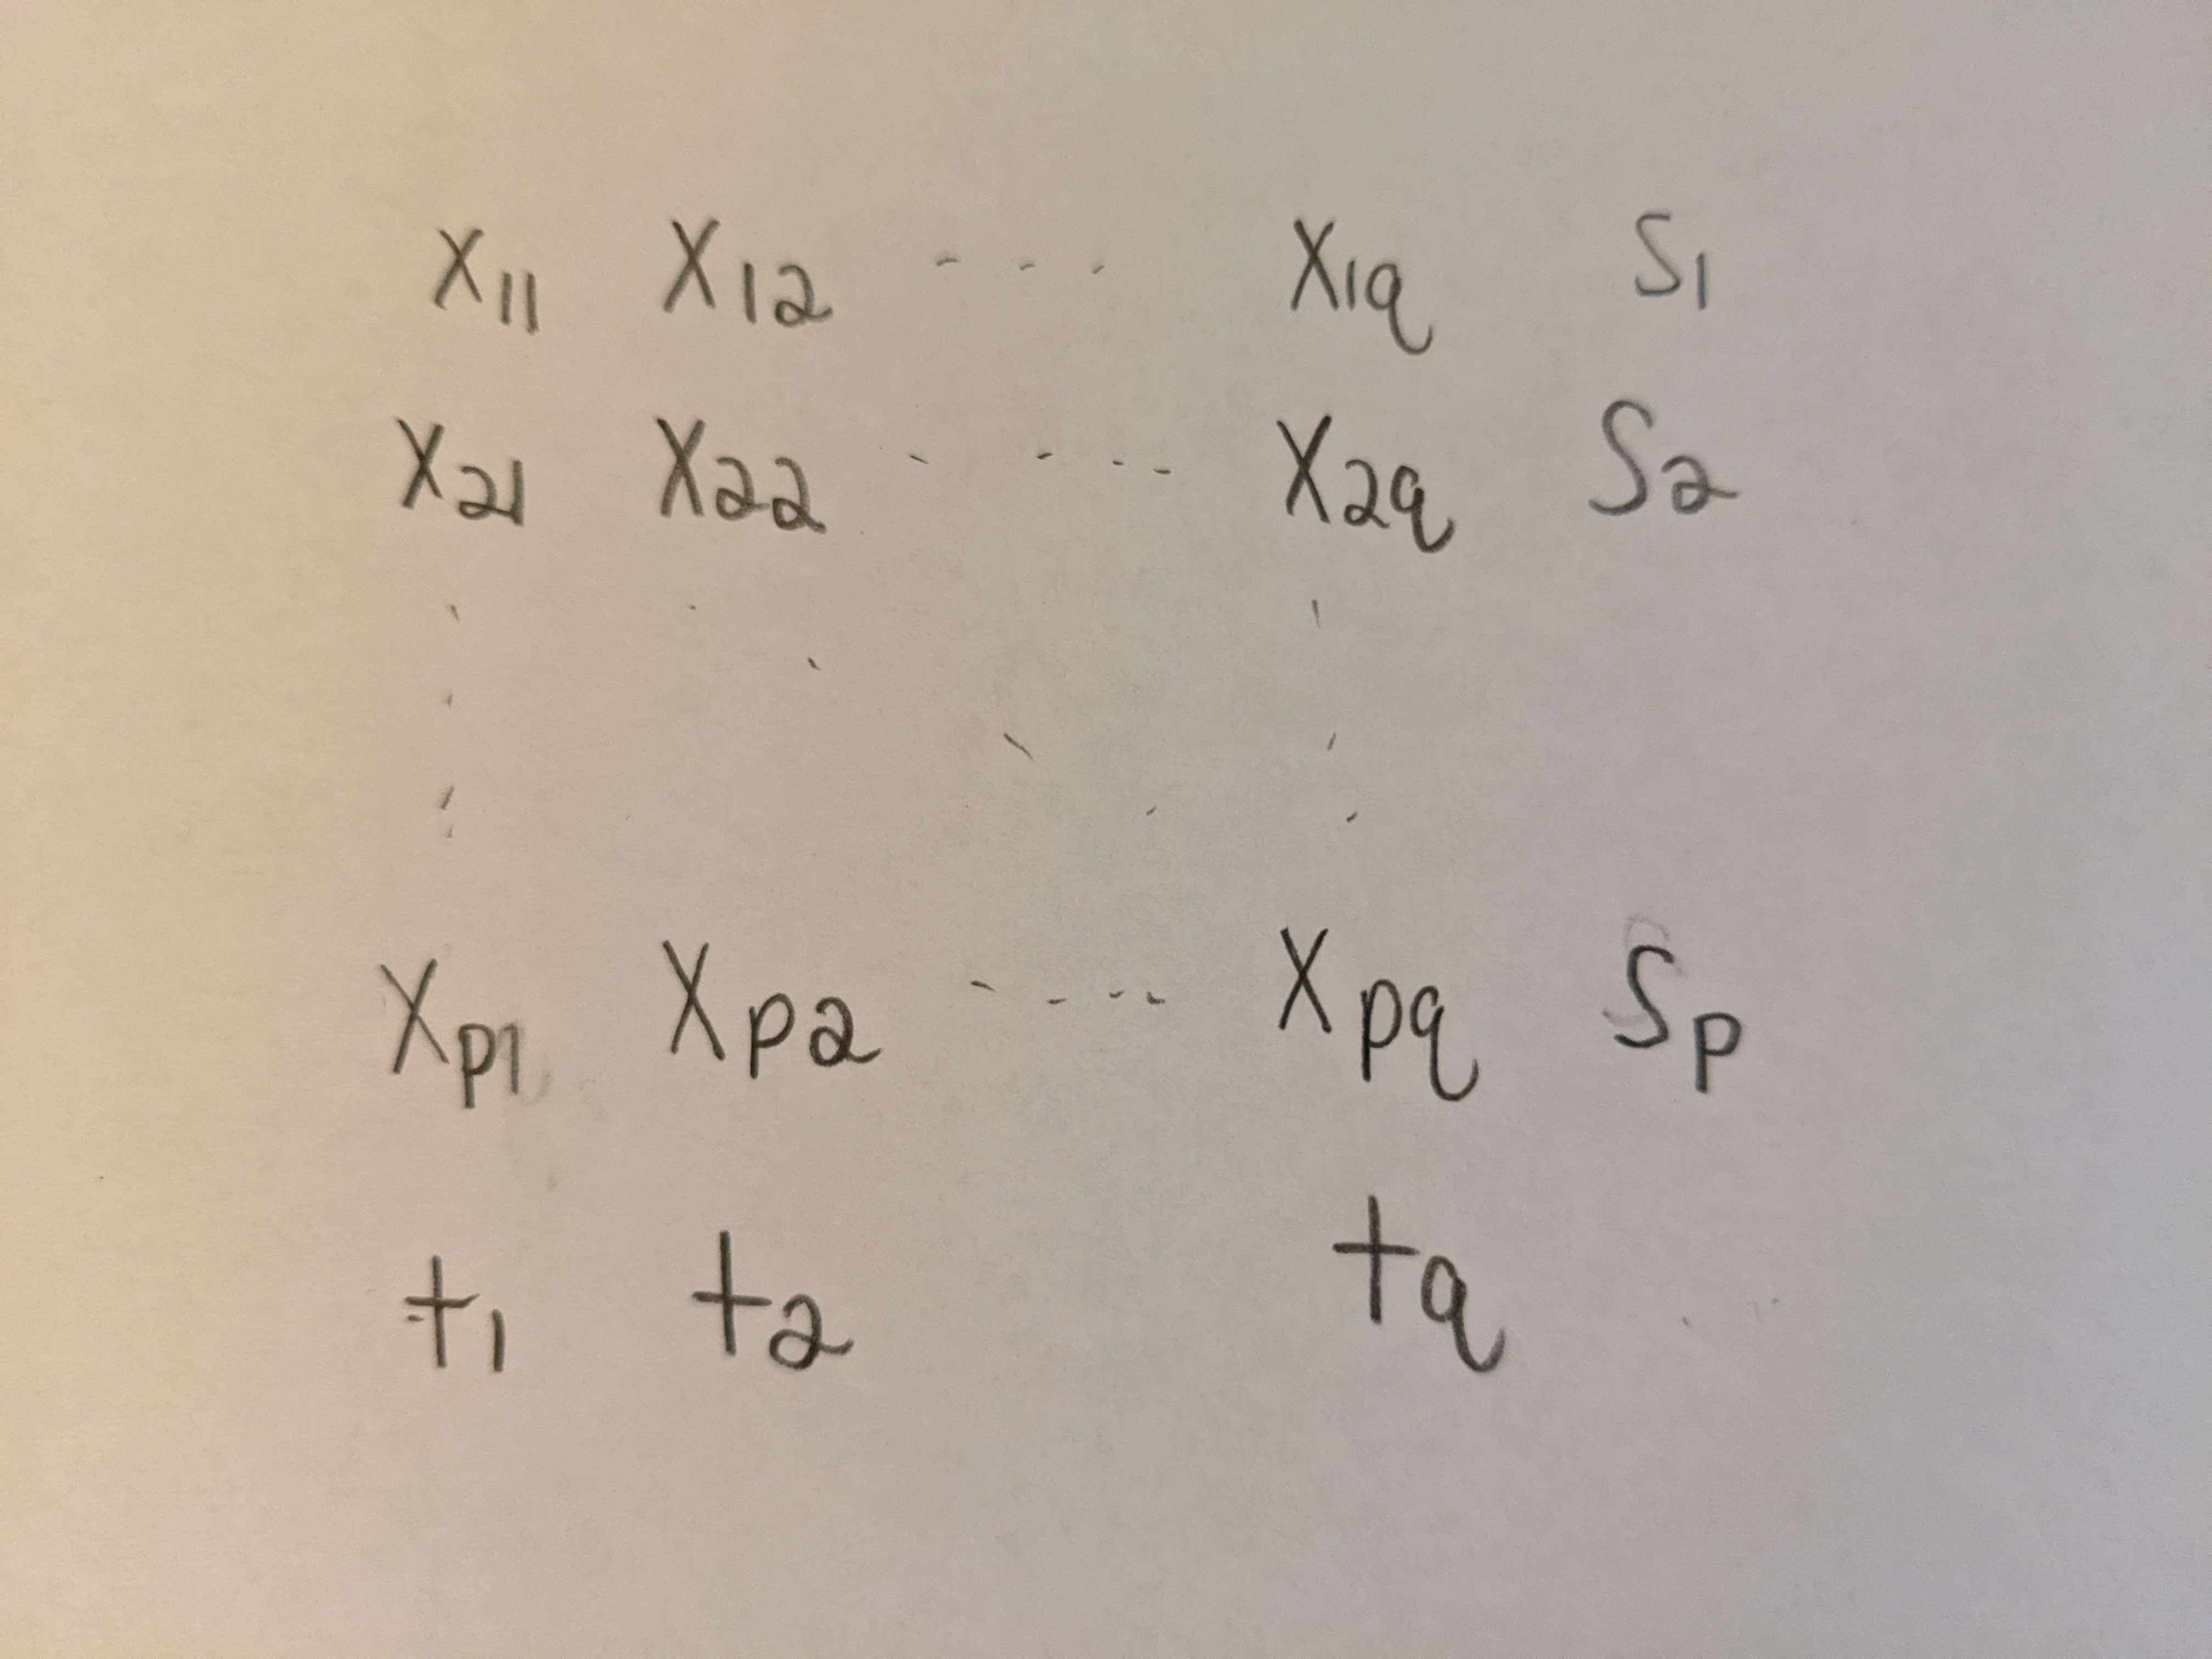
\includegraphics[width=\textwidth]{pic1}
%\end{figure}